\section{Hex-a-Hop}

\begin{frame}
	\frametitle{Hex-a-Hop}
	\begin{columns}
		\begin{column}{6cm}
			\begin{itemize}
				\item Hexagonal puzzle game
				\item<2-> Goal: Destroy all green tiles by walking on them
				\item<3-> Special tiles: Trampolines, turquoise tiles, high tiles
				\item<4-> Dynamic behavior depends on player's moves
			\end{itemize}
		\end{column}
		\begin{column}{5cm}
			\begin{figure}
				\centering
				\includegraphics[width=5cm]{images/hexahop.png}
			\end{figure}
		\end{column}
	\end{columns}
\end{frame}

\begin{frame}
	\frametitle{Encoding}
	\begin{block}{State space}
		\begin{itemize}	
			\item Boolean variables $v_{x,y}^{t}$ with $(x,y)$ position on field, $t$ time step
			\item Semantic: $v_{x,y}^{t} \equiv 1 \Leftrightarrow$ Player is at time step $t$ at position $(x,y)$
		\end{itemize}
	\end{block}
	\begin{itemize}
		\item $\forall t:$ Player has to be on exactly one tile
	\end{itemize}
\end{frame}

\begin{frame}
	\frametitle{Movement behavior}
	\begin{columns}
		\begin{column}{6cm}
			\begin{itemize}
				\item How to encode legal moves?
				\item<2-> $\forall x,y:$ calculate set of neighbors $N$
				\begin{displaymath}
					\bigwedge_{x,y,t} v_{x,y}^t \Rightarrow \bigvee_{n\in N} v_{n}^{t+1}
				\end{displaymath}
			\end{itemize}
		\end{column}
		\begin{column}{5cm}
			\begin{figure}
				\centering
				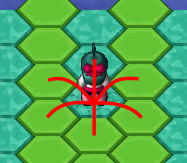
\includegraphics[width=5cm]{images/movement.png}
			\end{figure}
		\end{column}
	\end{columns}
\end{frame}

\begin{frame}
	\frametitle{Dynamic tiles}
	\begin{itemize}
		\item Tile behavior when visited
		\begin{displaymath}
			\text{Turquoise} \Rightarrow \text{Green} \Rightarrow \text{Destroyed}
		\end{displaymath}
		\item Dynamic type function
		\begin{displaymath}
			dT(\pmb x,t+1)=
			\begin{cases}
				dT(\pmb x, t) & v_{\pmb x}^{t} \not \equiv 1\\
				\text{Destroyed} & v_{\pmb x}^{t} \equiv 1 \wedge dT(\pmb x,t) = \text{Green}\\
				\text{Green} & v_{\pmb x}^{t} \equiv 1 \wedge dT(\pmb x,t)=\text{Turquoise}
			\end{cases}
		\end{displaymath}
	\end{itemize}
\end{frame}

\begin{frame}
	\frametitle{Start \& end condition}
	\begin{block}{Start condition}
		\begin{itemize}
			\item Add start position $\pmb x$ to clauses: $v_{\pmb x}^{0}$
		\end{itemize}
	\end{block}

	\begin{block}{End condition}
		\begin{itemize}
			\item All green tiles have to be destroyed
			\begin{displaymath}
				\bigwedge_{\pmb x} \neg (dT(\pmb x, T) = \text{Green})
			\end{displaymath}
			\item $T$ last timestep
		\end{itemize}
	\end{block}
\end{frame}

\begin{frame}
	\centering
	\hfill \Large Live demonstration \hfill\hfill
\end{frame}
